%*************************************************
% A template for PhD and MSc thesis. V1.0.
% Please see "guideline.pdf" first.
%*************************************************
% Iman Izadi, 1394
% Dept. of Electrical and Computer Engineering, IUT
%*************************************************
% این قالب بر اساس "شیوه‌نامه تدوین پایان‌نامه‌ها و رساله‌های 
%تحصیلات تکمیلی" دانشگاه صنعتی اصفهان تهیه شده است
%*************************************************

\documentclass[a4paper,fleqn]{report} 
%\usepackage{refcheck}

% All the packages and general definitions are included in this file: preamble.tex
%*************************************************
% All the packages and definitions are included here.
%*************************************************
%*************************************************
% Iman Izadi, 1394
% Dept. of Electrical and Computer Engineering, IUT
%*************************************************


\usepackage{array} % Load array package


\usepackage{amsthm,amssymb,amsmath}			% Writing math
\usepackage{epsf,graphicx}									% Including graphics
\usepackage[a4paper]{geometry}							% Fixing page layout and margins
\usepackage{titlesec}											% Change chapter and section titles
\usepackage{setspace}											% Change line spacing
\usepackage[stable,bottom]{footmisc}					% Move footnotes to the bottom of page

\usepackage{zref-perpage}									% Reset footnote counter in each page
\zmakeperpage[1]{footnote}

\usepackage{xepersian}										% Persian
\settextfont{XB Zar}												% Persian font
\usepackage{zref}


% Use English digits in equations
%\DefaultMathsDigits

% Default footnotes from left to right
\setfootnoteLR

% Use English numbers for English footnotes
\makeatletter
\def\@makeLTRfnmark{\hbox{\@textsuperscript{\latinfont\@thefnmark}}}
\renewcommand\@makefntext[1]{%
    \parindent 1em%
    \noindent
    \hb@xt@1.8em{\hss\if@RTL\@makefnmark\else\@makeLTRfnmark\fi}#1}
\makeatother

% Use dash instead of dot in section numbers
\SepMark{-}										

% Change fonts and margins of section and subsection titles
% For chapters please see firstpages.tex
\titlespacing*{\section}{0pt}{1cm}{0.2cm}
\titleformat{\section}
  {\fontsize{12}{6}\scshape\bfseries}{\thesection}{1em}{}

\titlespacing*{\subsection}{0pt}{.8cm}{0cm}
\titleformat{\subsection}
  {\fontsize{11}{6}\scshape\bfseries}{\thesubsection}{1em}{}
  
% Fix table of contents for chapters
\makeatletter 
\def\@chapter[#1]#2{\ifnum \c@secnumdepth >\m@ne
     \refstepcounter{chapter}%
     \typeout{\@chapapp\space\thechapter.}%
     \addcontentsline{toc}{chapter}%
       	{\@chapapp~\protect\numberline{\tartibi{chapter}\,:\space #1}}
  \else
  	 \addcontentsline{toc}{chapter}{#1}%
  \fi
  \chaptermark{#1}%
  \addtocontents{lof}{\protect\addvspace{10\p@}}%
  \addtocontents{lot}{\protect\addvspace{10\p@}}%
  \@makechapterhead{#2}%
  \@afterheading}
\makeatother
							

\begin{document}

% The first pages (before abstract) are included in this file: firstpages.tex
%*************************************************
% In this file the first few pages are typeset.
% Make the changes accordingly
%*************************************************

% شماره صفحات با حروف
\pagenumbering{adadi}

%***************************
% 1st page: Blank
%***************************
\thispagestyle{empty}
\mbox{}
\pagebreak

%***************************
% 2nd page: Besmelah
%***************************
\thispagestyle{empty}
\begin{center}
	~\vfill
	
\includegraphics[scale=1]{besm1.jpg}
	~\vfill
\end{center}
\pagebreak

%***************************
% 3rd page: Title
%***************************
\thispagestyle{empty}
%\pagenumbering{gobble}
\newgeometry{left=3cm,right=3cm,top=2cm}
\begin{center}

\includegraphics[height=3cm]{iut_logo.png}
\vspace{0.4cm}

\textbf{دانشگاه صنعتی اصفهان}\\
\vspace{0.4cm}

{\large

	دانشکده مهندسی برق و کامپیوتر
}
\vspace{3.5cm}

{\Large
	\textbf{تحلیل شبکه پیچیده از شبکه تراکنش   بیت‌کوین \cite{r0}}\\
}
\vspace{3.5cm}

{\Large
	گزارش پایانی درس ارائه مطلب\\
}
\vspace{1cm}

{\large
	\textbf{مسیح تنورساز}\\
}
\vspace{3.5cm}

{\large
	استاد درس\\
}
\vspace{0.5cm}

{\large
	\textbf{دکتر محمدحسین منشئی}\\
}
\vspace{4cm}

\textbf{1402}

\end{center}
\restoregeometry
\pagebreak

%***************************
% 4th page: Signatures
%***************************
\thispagestyle{empty}
\newgeometry{left=3cm,right=3cm,top=2cm}
\begin{center}

\includegraphics[height=3cm]{iut_logo.png}
\vspace{0.4cm}

\textbf{دانشگاه صنعتی اصفهان}\\
\vspace{0.4cm}

{\large
	دانشکده مهندسی برق و کامپیوتر
}
\vspace{1.8cm}

\vfill

{\Large
	گزارش پایانی درس ارائه مطلب -- آقای مسیح تنورساز\\
	\vspace{1.6cm}
	
}


\end{center}
{\Large
تحت عنوان\\
}

\vspace{0.3cm}

{\large
	\textbf{تحلیل شبکه پیچیده از شبکه تراکنش بیت‌کوین}
}

\vfill

\restoregeometry
\pagebreak

%***************************
% 5th page: Acknowledgment
%***************************
\thispagestyle{empty}
\newgeometry{left=3cm,right=4cm,top=4cm}
\vspace*{1.5cm}

{\large
	\textbf{تشکر و قدردانی}\\

	
پروردگار منّان را سپاسگزارم ......

}
\restoregeometry
\pagebreak

%***************************
% 8th page: Table of contents
%***************************

\titleformat{\chapter}[display]
	{\normalfont\LARGE\bfseries\centering}{\chaptertitlename ~ \tartibi{chapter}}{20pt}{\LARGE}
\newgeometry{left=2.5cm,right=3cm,top=3cm,bottom=2.5cm,includehead=false,headsep=1cm,footnotesep=.5cm}
\baselineskip=.7cm

\addtocontents{toc}{\textbf{\underline{عنوان}}}
\addtocontents{toc}{\hfill\textbf{\underline{صفحه}}\par}
\addcontentsline{toc}{section}{فهرست مطالب}
\tableofcontents
\pagebreak

\addcontentsline{toc}{section}{فهرست تصاویر}
\listoffigures
\pagebreak

\addcontentsline{toc}{section}{فهرست جداول}
\listoftables
\pagebreak

% change the font and margins of a chapter title
\titlespacing*{\chapter}{0pt}{3.5cm}{6cm}
\titleformat{\chapter}[display]
	{\normalfont\LARGE\bfseries\raggedright}{\chaptertitlename ~ \tartibi{chapter}}{20pt}{\LARGE}

% No page numbers on the first page of a chapter
\assignpagestyle{\chapter}{empty}
							

% The abstract of the paper goes here: abstract.tex
%*************************************************
% In this file the abstract is typeset.
% Make changes accordingly.
%*************************************************

\addcontentsline{toc}{section}{چکیده}
\newgeometry{left=2.5cm,right=3cm,top=3cm,bottom=2.5cm,includehead=false,headsep=1cm,footnotesep=.5cm}
\setcounter{page}{1}
\pagenumbering{arabic}						% شماره صفحات با عدد
\thispagestyle{empty}

~\vfill

~\subsection*{چکیده}
\begin{large}
\baselineskip=0.7cm
تحلیل شبکه‌های پیچیده\LTRfootnote { Complex Network } به عنوان یکی از شاخه‌های نوین علم شبکه‌ها، به بررسی ساختار و پویایی شبکه‌های پیچیده می‌پردازد. شبکه تراکنش بیت‌کوین\LTRfootnote { Bitcoin
Transaction Network }  به عنوان یکی از بزرگترین و مهم‌ترین شبکه‌های مالی دیجیتال، نمونه‌ای بارز از یک شبکه پیچیده است که تحلیل آن می‌تواند دیدگاه‌های ارزشمندی در مورد رفتار کاربران و ساختار کلان این شبکه فراهم کند. در این پژوهش، به بررسی شبکه تراکنش بیت‌کوین از جایگاه تحلیل شبکه‌های پیچیده پرداخته شده است.

در این مقاله، شبکه‌ی پیچیده‌ی تراکنش‌های بیت‌کوین را مورد بررسی و تحلیل قرار می‌دهیم. به‌طور خاص، یک روش نمونه‌گیری جدید به نام پیمایش تصادفی با بازگشت\LTRfootnote { Random Walk
With Flying-Back (RWFB)  } معرفی می‌شود تا نمونه‌گیری داده‌ها به‌طور موثرتری انجام شود. سپس، تحلیل جامعی از شبکه بلاکچین\LTRfootnote { Blockchain } بیت‌کوین از نظر توزیع درجه، ضریب خوشه‌بندی، طول کوتاه‌ترین مسیر، مولفه‌های متصل، مرکزیت، خودهمبستگی، و ضریب باشگاه ثروتمندان انجام می‌دهیم. پس از تحلیل، شاهد چندین نتیجه‌گیری جالب و حیرت انگیز مانند پدیده دنیای کوچک، وضعیت چند مرکزی، اتصال ترجیحی، و عدم تاثیر باشگاه ثروتمندان در شبکه فعلی خواهیم بود.


\vspace{0.5 cm}

\noindent\textbf{واژه‌های کلیدی:}
1- بیت‌کوین، 2- بلاکچین، 3- شبکه پیچیده، 4-تحلیل شبکه.
\end{large}

\vspace*{-10cm} % Add negative space to bring the content closer to the footnote								

%*****************************************************************
%% تنظیم مناسب صفحه و فونت برای متن اصلی پایان‌نامه
\newgeometry{left=2.5cm,right=3cm,top=3cm,bottom=2.5cm,includehead=false,headsep=1cm,footnotesep=.5cm}
\settextfont{XB Zar}\fontsize{13}{0}\selectfont
\setlatintextfont{Times New Roman}\fontsize{11}{6}
\baselineskip=.9cm

% Moving page number to top right
\pagestyle{myheadings}
%*****************************************************************

% Main chapters
% Chapter 1
\chapter{مقدمه}

در سال‌های اخیر، بیت‌کوین \cite{r1} به عنوان یکی از برجسته‌ترین ارزهای دیجیتال از زمان پیدایش آن در سال 2009 توسط ساتوشی ناکاموتو\LTRfootnote { Satoshi Nakamoto } مورد توجه قرار گرفته است. ویژگی‌های نوآورانه‌ای نظیر ناشناس بودن، کارمزد پایین تراکنش، عدم تمرکز و دسترسی دائمی به خدمات، بیت‌کوین را به موضوعی پرطرفدار در سال‌های گذشته تبدیل کرده است. با این حال، تحقیقات محدودی در زمینه تحلیل شبکه بیت‌کوین انجام شده است. تحلیل ساختار شبکه‌ تراکنش‌های بیت‌کوین از منظر شبکه‌های پیچیده بسیار مهم است زیرا می‌تواند رازهای سیستم‌های بلاکچین موجود را آشکار کند.

مهمترین مشارکت‌های این پژوهش به شرح زیر خلاصه می‌شود:

یک روش نمونه‌گیری جدید به نام پیمایش تصادفی با بازگشت برای تحلیل داده‌های تراکنش بیت‌کوین معرفی می‌گردد. روش بیان شده در حالی که پیچیدگی محاسباتی کمتری نسبت به روش های متعارف دارد، نمونه برداری\LTRfootnote { Sampling } دقیق‌تری از شبکه پیچیده بیت‌کوین ارائه می‌دهد و ویژگی‌های شبکه اصلی بیت‌کوین را حفظ می‌کند.
سپس با استفاده از روش معرفی شده، از شبکه نمونه برداری کرده و به تحلیل آن میپردازیم.
با تحلیل این شبکه پیچیده چندین مشاهده جدید از عملکرد کاربران و ساختار شبکه فعلی بیت‌کوین به دست می‌آوریم.

مشاهدات جدید درک عمیقی از ساختار شبکه بلاکچین بیت‌کوین ارائه می‌دهند و می‌توانند به بهبود امنیت و کارایی شبکه‌های بلاکچین ارزهای دیجیتال کمک کنند.
\section{مقدمه‌ای بر بلاکچین}
 
\begin{figure}[t]
\centering
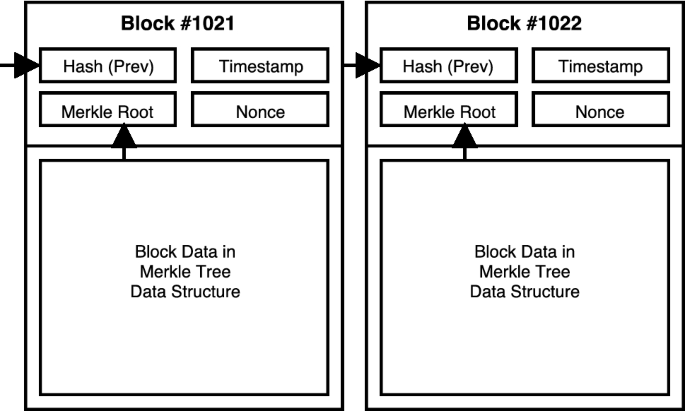
\includegraphics[height=7cm,width=10cm]{Blockchain.png}
\caption{ساختار کلی بلاکچین}
\label{bc}
\centering
\end{figure}
بلاکچین یک فناوری انقلابی است که به عنوان پایه‌ای برای بیت‌کوین و سایر ارزهای دیجیتال\LTRfootnote { Cryptocurrency } عمل می‌کند. در ساده‌ترین شکل، بلاکچین یک دفتر کل\LTRfootnote { Ledger }  توزیع شده و تغییرناپذیر است که تراکنش‌ها را به صورت امن و شفاف ذخیره می‌کند \cite{r2}.
\subsection{مفهوم بلاکچین}
همانطور که در شکل \ref{bc} قابل مشاهده است، ساختار بلاکچین شامل تعدادی بلاک می‌باشد که اطلاعات تراکنش‌ها رو درون خود جای داده اند و به کمک زنجیره‌ای به یکدیگر متصل شده اند. هر بلاک شامل اطلاعات زیر است:

\begin{itemize}
    \item \textbf{اطلاعات تراکنش‌ها:}  لیستی از تراکنش‌های انجام شده.
    \item \textbf{هش\footnote{ Hash } بلاک قبلی:} یک رشته منحصر به فرد که به بلاک قبلی اشاره می‌کند و بلاک‌ها را به یکدیگر متصل می‌سازد.
    \item \textbf{هش بلاک فعلی:} یک رشته منحصر به فرد که به محتوای بلاک اشاره دارد و با استفاده از الگوریتم‌های رمزنگاری ایجاد می‌شود.
\end{itemize}

\subsection{نحوه کار بلاکچین}

بلاکچین یک سیستم توزیع‌شده و غیرمتمرکز است که امکان ثبت و ذخیره‌سازی امن و شفاف اطلاعات را بدون نیاز به یک نهاد مرکزی فراهم می‌کند. در این بخش، نحوه کار بلاکچین را با جزئیات بیشتری بررسی می‌کنیم.

\subsubsection{تراکنش‌ها}
افراد تراکنش‌های خود را از طریق یک شبکه توزیع‌شده ارسال می‌کنند. هر تراکنش شامل اطلاعاتی نظیر فرستنده، گیرنده و مقدار ارز منتقل شده است. این تراکنش‌ها در شبکه منتشر می‌شوند تا توسط گره‌های\LTRfootnote { Node } موجود در شبکه بررسی و تایید شوند.

\subsubsection{تایید تراکنش‌ها}
تراکنش‌ها توسط گره‌های شبکه تایید می‌شوند. گره‌ها دستگاه‌هایی هستند که بلاکچین را پشتیبانی می‌کنند و مسئولیت تایید صحت تراکنش‌ها را بر عهده دارند. برای تایید تراکنش‌ها، گره‌ها از الگوریتم‌های رمزنگاری استفاده می‌کنند تا اطمینان حاصل کنند که فرستنده تراکنش واقعاً مالک ارز دیجیتال مورد نظر است.

\subsubsection{ایجاد بلاک جدید}
پس از تایید تراکنش‌ها، این تراکنش‌ها به یک بلاک جدید اضافه می‌شوند. هر بلاک شامل مجموعه‌ای از تراکنش‌های تایید شده است که به همراه یک شناسه یکتا (هش بلاک) و هش بلاک قبلی به بلاکچین اضافه می‌شود. فرآیند ایجاد بلاک جدید معمولاً توسط استخراج‌کنندگان\LTRfootnote { Miners }  انجام می‌شود که از قدرت محاسباتی خود برای حل مسائل پیچیده ریاضی استفاده می‌کنند.

\subsubsection{افزودن به زنجیره}
بلاک جدید به زنجیره بلاک‌های قبلی متصل می‌شود. این اتصال با استفاده از هش بلاک قبلی و هش بلاک جدید انجام می‌شود. هش بلاک جدید باید به گونه‌ای محاسبه شود که با معیارهای مشخصی سازگار باشد، که این امر به تضمین امنیت و یکپارچگی بلاکچین کمک می‌کند.

\subsubsection{توزیع بلاکچین}
نسخه جدید بلاکچین به تمام گره‌های شبکه ارسال می‌شود. پس از تایید و صحت سنجی بلاک، آنها نسخه‌های خود را به‌روزرسانی می‌کنند. این فرآیند به گره‌های موجود در شبکه اجازه می‌دهد تا از یک نسخه مشترک و به‌روز بلاکچین استفاده کنند. این امر باعث شفافیت شبکه و همچنین غیرمتمرکز بودن آن می‌شود.

\subsection{مزایای بلاکچین}

بلاکچین به عنوان یک فناوری نوآورانه دارای مزایا و کاربردهای فراوانی است که بهبودهای قابل توجهی در مقایسه با سیستم‌های سنتی ارائه می‌دهد. در این بخش، برخی از مهم‌ترین مزایای بلاکچین شرح داده می‌شوند.

\subsubsection{توزیع شدگی}
بلاکچین به صورت توزیع شده عمل می‌کند، به این معنا که داده‌ها در شبکه‌ای از گره‌ها ذخیره می‌شوند و هیچ نقطه متمرکزی برای حمله وجود ندارد. این ویژگی باعث افزایش مقاومت شبکه در برابر حملات سایبری و کاهش خطر از دست رفتن داده‌ها می‌شود.

\subsubsection{شفافیت}
یکی از ویژگی‌های بارز بلاکچین، شفافیت آن است. تمامی تراکنش‌ها در بلاکچین عمومی هستند و هر کسی می‌تواند آنها را مشاهده کند. این شفافیت موجب افزایش اعتماد کاربران و کاهش احتمال تقلب می‌شود.
هرچند که امروزه سیستم‌های خصوصی مبتنی بر بلاکچین نیز در حال گسترش و تولید اند.

\subsubsection{تغییرناپذیری}
تراکنش‌های ذخیره شده در بلاکچین قابل تغییر یا حذف نیستند. هر بلاک شامل هش بلاک قبلی است و این اتصال به زنجیره‌ای از بلاک‌ها منجر به تغییرناپذیری داده‌ها می‌شود. این ویژگی، از تغییرات غیرمجاز و دستکاری در داده‌ها جلوگیری می‌کند.

\subsubsection{امنیت}
بلاکچین از الگوریتم‌های رمزنگاری پیچیده برای ایجاد هش استفاده می‌کند که امنیت داده‌ها را تضمین می‌کند. هر تراکنش و بلاک توسط الگوریتم‌های رمزنگاری محافظت می‌شوند و این امر مانع از دسترسی غیرمجاز و هک شدن داده‌ها می‌شود.


\section{مقدمه‌ای بر شبکه‌های پیچیده} 
شبکه‌های پیچیده، به عنوان یک زیرشاخه مهم در علم شبکه‌ها، ساختارها و رفتارهای پیچیده‌ای را مدل‌سازی و بررسی می‌کنند. به دلیل پیچیدگی بالای موجود در اینگونه شبکه‌ها، تحلیل و مطالعه خواصشان نیازمند روش‌ها و تکنیک‌های منحصربه‌فرد می‌باشد. این شبکه‌ها معمولاً از عناصر متعدد و پیچیده‌ای مانند گره‌ها (نقاط) و پیوندها (لبه‌ها) تشکیل شده‌اند که با هم به شکل‌دهی ساختارهای غیرمنظم و پویایی منجر می‌شوند. این ساختار پیچیده با استفاده از گراف‌ها مدل می‌شود. از این رو تئوری گراف و بررسی ساختار شبکه‌های پیچیده، بسیار شباهت دارند.

شبکه‌های پیچیده در زندگی مدرن امروزی نقش مهمی ایفا می‌کنند. همچنین شاهد حضور پررنگ شبکه‌های پیچیده در زندگی روزمره انسان هستیم. یکی از این شبکه‌های پیچیده؛ شبکه تراکنش‌های بیت‌کوین، به عنوان یک رمزارز مورد استفاده توسط مردم می‌باشد.

\subsection{ویژگی‌های شبکه‌های پیچیده}
برای بررسی و آشنایی با شبکه‌های پیچیده، نیازمند شناخت ویژگی‌ها و خصوصیات اینگونه شبکه‌ها می‌باشیم.

در ادامه به بررسی اجمالی ویژگی‌های یک شبکه پیچیده می‌پردازیم.
\begin{itemize}
    \item \textbf{تعداد زیاد گره‌ها و پیوندها:} شبکه‌های پیچیده معمولاً شامل تعداد زیادی گره و پیوند هستند. به عنوان مثال، در شبکه‌های اجتماعی، گره‌ها نماینده افراد و پیوندها نماینده روابط اجتماعی بین آن‌ها هستند و یا در شبکه پیچیده بیت‌کوین، آدرس‌های تراکنش نماینده گره‌ها و تراکنش انجام شده میان آدرس مبدا و آدرس مقصد نمایانگر پیوند جهت‌دار و وزن‌دار میان دو گره می‌باشد.
    
    \item \textbf{ساختار غیرمنظم:} شبکه‌های پیچیده دارای ساختاری غیرمنظم و پیچیده هستند. این ساختار به دلیل تعداد بالای پیوندها و پویایی شبکه، به صورت مرتب و منظم نیست. به عبارت دیگر، الگوی خاصی برای چگونگی اتصال گره‌ها به یکدیگر وجود ندارد و شبکه‌ها به صورت تصادفی و پویا تغییر می‌کنند.
    
    \item \textbf{همبستگی و ساختارهای سلسله‌مراتبی:} شبکه‌های پیچیده ممکن است دارای همبستگی‌ها و ساختارهای سلسله‌مراتبی باشند. این به این معناست که برخی از گره‌ها به عنوان گره‌های اصلی یا مرکزی عمل می‌کنند و بسیاری از گره‌های دیگر به این گره‌های مرکزی متصل می‌شوند.
\end{itemize}

\pagebreak

~\section{ساختار شبکه بیت‌کوین\footnote{ Bitcoin Network Construction }}
\begin{figure}[t]
\centering
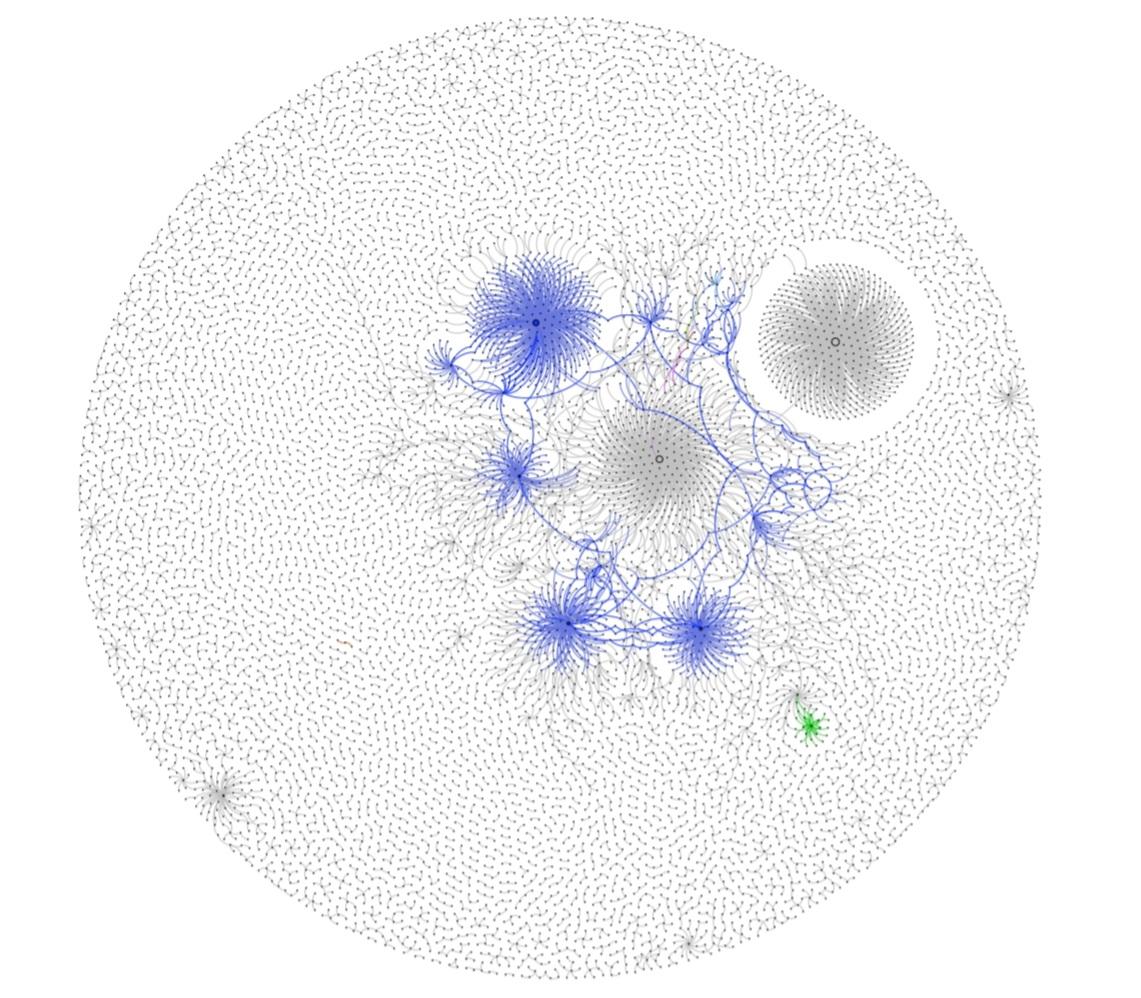
\includegraphics[height=6cm,width=7.5cm]{BTC_VISUAL.jpg}
\caption{نمایی از شبکه تراکنش بیت‌کوین با 10,000 گره منتخب \cite{r0}}
\label{btcv}
\centering
\end{figure}
این مقاله به بررسی تراکنش‌های بیت‌کوین پرداخته است که در آن، هر تراکنش می‌تواند چندین آدرس ورودی و چندین آدرس خروجی داشته باشد. به عنوان مثال، یک تراکنش از $x$ آدرس ورودی و $y$ آدرس خروجی استخراج می‌شود و به صورت $x \times y$ نمایش داده می‌شود. سپس، هر گره نماینده یک آدرس بیت‌کوین خواهد بود، همچنین هر لبه جهت‌دار نشان‌دهنده جهت انجام آن تراکنش است و وزن لبه متناسب با ارزش تراکنش مشخص می‌شود.

مقاله یک شبکه تراکنش بیت‌کوین را به یک گراف جهت‌دار وزنی تبدیل می‌کند که با \mbox{$G = (V, E, W)$} نشان داده می‌شود، جایی که $V$ مجموعه گره‌ها، $E$ مجموعه لبه‌ها و $W$ مجموعه وزن‌ها است. هر لبه به صورت $e_{ij} = (i, j, w_{ij})$ نمایش داده می‌شود. مجموعه $E$ با $N$ گره می‌تواند به صورت یک ماتریس $N \times N$ نمایش داده شود که اساساً یک ماتریس مجاورت است و با $A$ نشان داده می‌شود. برای هر عنصر $a_{ij}$ در $A$، داریم:

\[
a_{ij} = 
\begin{cases} 
w_{ij} & \text{ تعریف شده باشد} e_{ij} \text{اگر }  \\ 
0 & \text{در غیر این صورت} 
\end{cases}
\]
\newpage
داده‌های مورد استفاده در این مقاله؛ از تراکنش‌ها و آدرس تراکنش‌های موجود در پایگاه داده پروژه بیت‌کوین، از ژانویه 2017 تا ژانویه 2018 بدست آمده اند که شامل بیش از 148,000,000 گره و 870,000,000 لبه می‌باشند. شکل \ref{btcv} نمایی از شبکه تراکنش بیت‌کوین با 10,000 گره منتخب را نشان می‌دهد.

\section{نمونه‌برداری از شبکه بیت‌کوین}

شبکه تراکنش بیت‌کوین یک گراف بسیار بزرگ با میلیون‌ها گره است، بنابراین لازم است که یک شبکه نمونه، نماینده، برای ساده‌سازی تحلیل‌ها بدست آوریم. برخی از مطالعات قبلی نشان داده‌اند که روش‌های نمونه‌برداری مبتنی بر پیاده‌روی تصادفی\footnote{ Random walk(RW)} می‌توانند خواص ساختاری شبکه بلاکچین مقیاس آزاد\footnote{Scale-free} را به خوبی حفظ کنند. بنابراین، در این مقاله نیز یک روش نمونه‌برداری گراف، مبتنی بر پیاده‌روی تصادفی، برای نمایندگی شبکه بلاکچین بیت‌کوین طراحی معرفی می‌گردد.

\subsection{روش نمونه برداری RWFB}
در روش‌های سنتی پیاده‌روی تصادفی، گره بعدی $j$ به صورت تصادفی از همسایگان گره فعلی $i$ انتخاب می‌شود. با این حال، این روش‌ها نمی‌توانند به دقت شبکه بیت‌کوین را نمونه‌برداری کنند. برای رفع این مشکل، روش ابداعی با نام پیاده روی تصادفی با بازگشت به عقب طراحی و معرفی می‌گردد.

به طور خاص، پیاده روی تصادفی با بازگشت به عقب هنگام نمونه‌برداری از شبکه، احتمال بازگشت به گره فعلی را نیز در نظر می‌گیرد. در هر گام از پیاده‌روی تصادفی جهت‌دار، RWFB با احتمال بازگشت $p$ به گره فعلی یعنی $i$ بازمی‌گردد؛ و با احتمال $1 - p$ یک همسایه تصادفی از میان $k_i$ همسایه‌های خود را انتخاب می‌کند، بنابراین هر کدام دارای احتمالی برابر با $(1 - p) / k_i$ هستند. احتمال RWFB را که با $P_{RWFB_i}$ نشان داده می‌شود، به صورت زیر تعریف می‌کنیم:
\[
P_{RWFB_i} = 
\begin{cases} 
p & \text{بازگشت به گره $i$} \\
\frac{1 - p}{k_i} & \text{انتقال به همسایه $j$ از گره $i$ }
\end{cases}
\]
\\
پیاده‌روی همیشه از یک گره تصادفی شروع می‌شود. علاوه بر این، اگر در طول پیاده‌روی به بن‌بست برخورد کند، یک گره تصادفی دیگر برای ادامه انتخاب می‌شود تا زمانی که اندازه نمونه‌برداری به مقدار دلخواه و موردنیازمان برسد.



حال پس از اتمام نمونه‌برداری نیاز به تعریف گراف جدید داریم. گراف نمونه‌برداری شده با تابع بازگشت را به عنوان $G_{RWFB} = (V_i, E_{i,j}, w_{i,j})$ دوباره تعریف می‌کنیم. در این گراف جهت‌دار و وزن‌دار، گره‌ها همان رئوس پیموده شده هستند و لبه‌ها همان گام‌هایی اند که پیموده ایم.


\subsection{ارزیابی روش نمونه‌برداری RWFB}
جدول ~\ref{eval}، مقایسه روش‌های نمونه‌برداری با استفاده از آماره D-statistic K-S را نشان می‌دهد.
این آماره مشخص می‌کند که ورودی هایش در معیارهای مختلف چه‌قدر متفاوت اند. هرچه تفاوت دو ورودی اش، که گراف نیز می‌باشند، بیشتر باشد عدد حاصل به یک نزدیکتر است.
هرچه عدد حاصل به صفر نزدیکتر باشد یعنی تفاوت میان گراف نمونه\footnote{$G_{RWFB} = (V_i, E_{i,j}, w_{i,j})$} و گراف اصلی\footnote{$G = (V, E, W)$} کمتر بوده است.

مطابق با جدول ~\ref{eval} می‌توان نتیجه گرفت؛ روش ابداعی عملکرد بهتری را نسبت به سایر روش‌های سنتی داشته است، گراف اصلی را بهتر نمونه‌برداری کرده و دارای خواص نسبتا مشابه با آن می‌باشد.
\begin{table}[t]
\centering
\begin{LTR}
\begin{latin}
\begin{tabular}{cccccc}
\hline
\textbf{Sampling Method} & \textbf{Degree} & \textbf{Clustering} & \textbf{Betweenness} & \textbf{Closeness} & \textbf{Average} \\
\hline
\textbf{RWFB} & 0.120 & 0.045 & 0.091 & 0.429 & \textbf{0.171} \\
RWS & 0.293 & 0.046 & 0.536 & 0.618 & 0.373 \\
RN & 0.895 & 0.053 & 0.151 & 0.433 & 0.383 \\
RE & 0.275 & 1.000 & 0.067 & 0.549 & 0.473 \\
FF & 0.187 & 1.000 & 0.075 & 0.669 & 0.483 \\
SB & 0.409 & 0.025 & 0.583 & 0.645 & 0.415 \\
\hline
\end{tabular}
\end{latin}
\end{LTR}
\caption{مقایسه روش‌های نمونه‌برداری با استفاده از  D-statistic K-S}
\label{eval}
\end{table}



% Chapter 2
\chapter{تحلیل شبکه‌های پیچیده}
\section{توزیع درجه\footnote{Degree distribution}}
بررسی توزیع درجه گره‌ها در شبکه بیت‌کوین بسیار حائز اهمیت است. درجه یک گره که با \(k\) نشان داده می‌شود، تعداد یال‌های مجاور آن گره را مشخص می‌کند. در شبکه تراکنش‌های بیت‌کوین، درجه \(k\) برای هر آدرس بیت‌کوین با مجموع تعداد تراکنش‌ها محاسبه می‌شود. تعداد تراکنش‌های ورودی (دریافت بیت‌کوین) به عنوان درجه ورودی و تعداد تراکنش‌های خروجی (پرداخت بیت‌کوین) به عنوان درجه خروجی شناخته می‌شود. توزیع درجه که با \(P(k)\) نشان داده می‌شود، احتمال این است که یک گره انتخابی به صورت تصادفی دارای درجه برابر با \(k\) باشد. اگر درجه \(k\) از قانون توان تبعیت کند، آنگاه \(P(k) \propto k^{-\alpha}\) است، که \(\alpha\) پارامتر مقیاس توزیع قانون توان است.

نتایج نشان می‌دهند که تمامی توزیع‌های درجه از قانون توان با دنباله‌های سنگین تبعیت می‌کنند. این نشان می‌دهد که شبکه بیت‌کوین یک شبکه مقیاس آزاد است که در آن تنها تعداد کمی از گره‌ها دارای تعداد زیادی اتصالات هستند در حالی که بیشتر گره‌ها دارای درجه‌های کم و اتصالات کمتری هستند. این یافته‌ها با نتایج تحقیقاتی که با داده‌های واقعی شبکه به دست آمده‌اند، سازگار است. 


\section{ضریب خوشه‌بندی و طول کوتاه‌ترین مسیر\footnote{Clustering coefficient and the shortest-path length}}

ضریب خوشه‌بندی و طول کوتاه‌ترین مسیر می‌توانند شبکه را از دیدگاه هندسی مورد ارزیابی قرار دهند. ضریب خوشه‌بندی متوسط شبکه با \(C\) نشان داده می‌شود که به صورت زیر تعریف می‌شود:
\[
C = \frac{1}{N} \sum_{i \in V(G)} \frac{\Delta_i}{k_i (k_i - 1) / 2},
\]
که در آن \(N\) تعداد گره‌ها، \(\Delta_i\) تعداد مثلث‌های کامل و \(k_i\) درجه گره \(i\) را نشان می‌دهند.

از سوی دیگر، طول متوسط کوتاه‌ترین مسیر با \(L\) نشان داده می‌شود که به صورت زیر تعریف می‌شود:
\[
L = \sum_{i,j \in V(G)}  \frac{l(i,j)}{N(N-1)},
\]
که در آن \(V(G)\) مجموعه گره‌های گراف \(G\) و \(l(i,j)\) طول کوتاه‌ترین مسیر بین \(i\) و \(j\) است. برای گراف تراکنش بیت‌کوین، ضریب خوشه‌بندی \(C_{Bitcoin} = 0.0071\) و طول کوتاه‌ترین مسیر \(L_{Bitcoin} = 3.833\) می‌باشد که نشان‌دهنده تعداد زیاد تراکنش‌های غیرمستقیم است.

\subsection{اثر جهان کوچک در شبکه بیت‌کوین\footnote{Small-world effect}}

اثر جهان کوچک یک ویژگی در شبکه‌های پیچیده است که نشان می‌دهد چگونه هر دو گره در یک شبکه بزرگ می‌توانند با تعداد کمی یال به یکدیگر متصل شوند. دو ویژگی اصلی شبکه‌های جهان کوچک عبارتند از:

\begin{itemize}
    \item \textbf{ضریب خوشه‌بندی بالا:} ضریب خوشه‌بندی نشان می‌دهد که چقدر احتمال دارد که دو گره همسایه یک گره دیگر نیز با هم متصل باشند. ضریب خوشه‌بندی بالا نشان‌دهنده وجود خوشه‌های محکم از گره‌ها است.
    \item \textbf{میانگین طول کوتاه‌ترین مسیر کم:} این ویژگی نشان می‌دهد که به طور میانگین، چند یال باید طی شود تا از یک گره به هر گره دیگر در شبکه رسید. در شبکه‌های جهان کوچک، این میانگین طول کوتاه است.
\end{itemize}

در شبکه بیت‌کوین، ضریب خوشه‌بندی و طول کوتاه‌ترین مسیر به صورت زیر محاسبه شده است:

\[
C_{\text{Bitcoin}} = 0.0071 \quad \text{و} \quad L_{\text{Bitcoin}} = 3.833
\]

این مقادیر نشان‌دهنده این است که شبکه بیت‌کوین دارای خوشه‌های محکم از گره‌ها و همچنین مسیرهای کوتاه بین گره‌ها است. بنابراین در شبکه پیچیده بیت‌کوین شاهد اثر جهان کوچک می‌باشیم. این اثر به این معناست که توکن‌های بیت‌کوین\footnote{Bitcoin tokens} می‌توانند در چند مرحله به اکثر گره‌ها منتقل شوند.

~\vfill
\section{مولفه‌های متصل\footnote{Connected component}}
با توجه به اینکه شبکه بلاکچین بیت‌کوین یک شبکه جهان کوچک است، تحلیل اتصال‌پذیری آن اهمیت زیادی دارد. در یک شبکه پیچیده، اگر هر جفت گره در یک زیرگراف حداقل یک مسیر متصل داشته باشد، آن زیرگراف را یک مولفه متصل می‌نامیم. در شبکه‌های جهت‌دار، مولفه‌های قویاً متصل\footnote{Strongly Connected Component(SCC)} به زیرگراف‌هایی اشاره دارد که هر جفت گره \text{($i , j$)} دارای مسیری جهت‌دار از $i$ به $j$ و از $j$ به $i$ به‌طور همزمان هستند. به‌طور مشابه، مولفه‌های ضعیفاً متصل\footnote{Weakly Connected Component(WCC)} به مولفه‌های متصل بدون جهت اشاره دارد.

نتایج حاصل از این تحلیل نشان می‌دهند که گراف شبکه پیچیده بیت‌کوین یک گراف نسبتا متصل است. همچنین احتمالاً گره‌های رابط، تعداد بسیاری از گره‌های جدا شده و منفرد را به شبکه متصل می‌کنند. در واقعیت، چنین گره‌های رابطی ممکن است صرافی‌ها، موسسات تجاری یا سازمان‌های مالی باشند. همچنین می‌توان نتیجه گرفت که بسیاری از تراکنش‌ها در این گراف تنها یک‌طرفه هستند. به عبارت دیگر، اکثر گره‌ها به‌طور مکرر تراکنش‌های دوطرفه (ورودی و خروجی) انجام نمی‌دهند و فقط بیت‌کوین پرداخت می‌کنند یا دریافت می‌کنند.



~\section{مرکزیّت\footnote{Centrality}}
تحلیل مولفه‌های متصل باعث شد به وجود گره‌های رابط پی ببریم. برای تأیید این فرضیه، مرکزیّت شبکه را تحلیل می‌کنیم.

~\subsection{مرکزیّت شبکه}
مرکزیّت شبکه مفهومی است که برای اندازه‌گیری اهمیت نسبی گره‌ها در یک شبکه استفاده می‌شود. این مفهوم به ما کمک می‌کند تا بفهمیم کدام گره‌ها نقش کلیدی‌تری در ساختار شبکه ایفا می‌کنند. در ادامه به بررسی چند نوع مرکزیّت در شبکه‌های پیچیده می‌پردازیم.

\subsubsection{مرکزیّت نزدیکی\footnote{Closeness centrality }}
مرکزیّت نزدیکی معیاری است که نشان می‌دهد یک گره چقدر به سایر گره‌های شبکه نزدیک است. این معیار بر اساس طول کوتاه‌ترین مسیرها از یک گره به سایر گره‌ها محاسبه می‌شود. فرمول مرکزیّت نزدیکی یک گره $i$ به صورت زیر است:
\[
O(i) = \frac{n-1}{\sum_{j=1}^{n-1} d(i, j)}
\]
که در آن $n$ تعداد گره‌های قابل دسترس گره $i$ و $d(j, i)$ فاصله کوتاه‌ترین مسیر بین گره $j$ و گره $i$ است. این معیار نشان می‌دهد که یک گره چقدر سریع می‌تواند به سایر گره‌ها دسترسی پیدا کند.

\subsubsection{مرکزیّت بینابینی\footnote{Betweenness centrality}}
مرکزیّت بینابینی نشان می‌دهد که یک گره چقدر در مسیرهای کوتاه بین سایر گره‌ها قرار دارد. این معیار نشان می‌دهد که یک گره چقدر در انتقال اطلاعات بین سایر گره‌ها نقش دارد. فرمول مرکزیّت بینابینی یک گره $i$ به صورت زیر است:
\[
B(i) = \sum_{u, v \in V} \frac{\sigma(u, v | i)}{\sigma(u, v)}
\]
که در آن $\sigma(u, v)$ تعداد کل مسیرهای کوتاه بین گره‌های $u$ و $v$ و $\sigma(u, v | i)$ تعداد مسیرهایی است که از گره $i$ عبور می‌کنند. این معیار نشان می‌دهد که یک گره چقدر در اتصال سایر گره‌ها به هم نقش دارد.
\\
\\
مطابق با یافته‌های این مقاله، مرکزیّت بینابینی با افزایش درجه گره افزایش می‌یابد. اگر تعداد زیادی از گره‌ها دارای مقادیر بالای بینابینی باشند، تعداد زیادی از گره‌های رابط در گراف ظاهر می‌شوند که باعث شکنندگی گراف می‌شود. این نتایج نشان می‌دهد که تعداد زیادی از گره‌های رابط در شبکه بیت‌کوین وجود ندارد و این شبکه در مقابل حذف گره‌ها مقاوم است. بیشتر گره‌ها دارای مقادیر نسبتاً کم نزدیکی و بینابینی هستند که نشان می‌دهد تعداد کمی گره‌های مرکزی وجود دارند. بنابراین، ما یک گراف چندمرکزی مشاهده می‌کنیم که در آن برخی از گره‌های مرکزی مستقیماً با تعداد زیادی از گره‌ها بدون واسطه متصل هستند. دلیل چندمرکزی و مقاومت عالی را می‌توان به توزیع ناهمگن گره‌ها نسبت داد که در بخش‌های بعدی مورد بررسی قرار می‌گیرد.


\section{عدم تناسب\footnote{Disassortativity}}
در این تحلیل تمایلات اتصالات شبکه بیت‌کوین مورد بررسی قرار گرفته است. محققان از ضریب همبستگی پیرسون\footnote{Pearson correlation coefficient} با نماد $\rho$ برای مشخص کردن تناسب شبکه استفاده کرده‌اند.

% این ضریب به‌شکل زیر محاسبه می‌شود:
%\begin{equation}
%\rho = \frac{\sum_{e_{ij} \in E(G)} (k_i k_j - \frac{1}{2}(k_i + k_j))^2}{\sum_{e_{ij} \in E(G)} \frac{1}{2}(k_i^2 + k_j^2) - \left( \sum_{e_{ij} \in E(G)} \frac{1}{2}(k_i + k_j) \right)^2}
%\end{equation}

نتیجه به‌دست آمده برای ضریب همبستگی پیرسون $\rho = -0.023$ بوده که نشان‌دهنده این است که شبکه دارای خاصیت عدم تناسب است. مطالعات قبلی بر روی ساختار شبکه بیت‌کوین نیز این موضوع را تایید می‌کنند.

درنهایت می‌توان نتیجه گرفت که گره‌های با درجه بالا ترجیح می‌دهند به گره‌های با درجه کمتر متصل شوند، درحالی‌که گره‌های با درجه پایین نیز ترجیح دارند به گره‌های با درجه بالاتر متصل شوند.
به عنوان مثال، گره‌های تازه وارد ترجیح می‌دهند با گره‌های درجه بالا (که احتمالا صرافی ها و غیره می‌باشند) متصل شوند.


\section{ضریب باشگاه ثروت‌مندان\footnote{Rich-club coefficient}}
پدیده باشگاه ثروتمندان در شبکه‌های پیچیده به پدیده‌ای اطلاق می‌شود که ارتباطات قوی بین گره‌های با درجه‌های بالا را نشان می‌دهد، به‌طوری‌که این گره‌ها به صورت زیرگروه‌هایی به نام "باشگاه‌های ثروتمندان" با هم ارتباط‌ برقرار می‌کنند.

ضریب باشگاه ثروتمندان $\phi(k)$ به عنوان یک معیار برای ارزیابی این پدیده تعریف می‌شود. این ضریب نسبت تعداد لینک‌های واقعی بین گره‌هایی را که درجه آن‌ها بیشتر از $k$ است به تعداد لینک‌های حداکثر ممکن بین این گره‌ها در شبکه با $N$ گره نشان می‌دهد:
\[
\phi(k) = \frac{2E>k}{N>k (N>k - 1)},
\]
که در آن $N>k$ تعداد کل گره‌هایی است که درجه آن‌ها بیشتر از $k$ است و $E>k$ تعداد یال‌های بین گره‌های $N>k$ است. $N>k (N>k - 1)/2$ حداکثر یال‌های ممکن بین تمام گره‌های $N>k$ است.

برای ارزیابی دقیق‌تر، از ضریب باشگاه ثروت‌مند نرمال‌شده $\phi_{\text{norm}}(k)$ استفاده می‌کنیم که به صورت زیر تعریف می‌شود:
\[
\phi_{\text{norm}}(k) = \frac{\phi(k)}{\phi_{\text{rand}}(k)},
\]
که در آن $\phi_{\text{rand}}(k)$ ضریب باشگاه ثروت‌مندان با توزیع درجه مشابه است. نتایج نشان می‌دهد که در اکثر ارزش‌های $k$، چیدمان باشگاه ثروت‌مندان وجود ندارد.

در کل، شبکه بیت‌کوین پدیده عدم وجود باشگاه ثروت‌مند را از خود نشان می‌دهد، که نشان‌دهنده آن است که گره‌های مرکزی با درجه بالا در این شبکه تمایل به اتصال با یکدیگر ندارند و در زیرگراف‌های متصل مختلف پخش می‌شوند. این اثر می‌تواند توسط واقعیت توضیح داده شود که گره‌های مرکزی احتمالاً تبادلات متداولی را انجام می‌دهند. در نتیجه، گره‌های ثروتمند در شبکه بیت‌کوین به طور مستقیم با یکدیگر ارتباط ندارند.

%%%%%%%%%%%%%%%%%%%%%%%%%%%%%
\chapter{جمع‌بندی}
\section{نتایج}

در این مقاله، ما به تحلیل شبکه‌های پیچیده بر روی شبکه تراکنش‌های بیت‌کوین پرداختیم. به طور خاص، یک روش نمونه‌برداری جدید با نام \textit{پیاده‌روی تصادفی با بازگشت به عقب} طراحی کرده‌ایم و از طریق تحلیل گراف‌های نمونه‌برداری شده، مشاهدات مهمی به‌دست آورده‌ایم.

ابتدا، توزیع درجه شبکه تراکنش‌های بیت‌کوین به توزیع قانون توان با دنباله سنگین تطابق دارد که به یک شبکه مقیاس آزاد نزدیک است. دوم، با تحلیل ضریب خوشه‌بندی میانگین، طول کوتاه‌ترین مسیر و اندازه‌گیری شبکه جهان کوچک، اطمینان حاصل کردیم که شبکه تراکنش‌های بیت‌کوین یک شبکه جهان کوچک است. سوم، از طریق تحلیل اجزای متصل، دریافتیم که بیشتر تراکنش‌ها به صورت معاملات یک‌طرفه هستند. علاوه بر این، مشاهده کردیم که شبکه بیت‌کوین یک شبکه چندمرکزی مقاوم در برابر حذف گره‌ها است. 

پس از آن، با توجه به ناهماهنگی شبکه بیت‌کوین، دریافتیم که گره‌های با درجه پایین تمایل به اتصال به گره‌های با درجات بالاتر دارند. در نهایت، شبکه تراکنش‌های بیت‌کوین فعلی پدیده باشگاه ثروتمندان را نشان نمی‌دهد. این یافته‌ها می‌تواند به ما در درک بهتر رفتارهای ساختاری شبکه‌های بلاکچین کمک کند. علاوه بر این، روش‌های تحلیل و الگوریتم‌های نمونه‌برداری نیز می‌توانند در فهم شبکه‌هایی با خصوصیات مشابه، مانند شبکه‌های مقیاس آزاد، شبکه‌های جهان کوچک و شبکه‌های ناهماهنگ، بینش‌های ارزشمندی ارائه ‌دهند.


% Appendices
\appendix
%% Appendix 1
%\chapter{}
%

% References
\renewcommand{\bibname}{مراجع}
\addcontentsline{toc}{section}{مراجع}

\begin{thebibliography}{99}

\begin{latin}

\baselineskip=.7cm

\bibitem{r0}
\noindent B. Tao, H. -N. Dai, J. Wu, I. W. -H. Ho, Z. Zheng and C. F. Cheang, "Complex Network Analysis of the
Bitcoin Transaction Network," in IEEE Transactions on Circuits and Systems II: Express Briefs., vol. 69,
no. 3, pp. 1009-1013, March. 2022

\bibitem{r1}
\noindent S. Nakamoto, “Bitcoin: a Peer-to-Peer Electronic Cash System,” Oct. 2008. [Online]. Available:
https://bitcoin.org/bitcoin.pdf

\bibitem{r2}
\noindent Z. Zheng, S. Xie, H. Dai, X. Chen and H. Wang, "An Overview of Blockchain Technology: Architecture,
Consensus, and Future Trends," 2017 IEEE International Congress on Big Data (BigData Congress),
Honolulu, HI, USA, 2017, pp. 557-564.


\end{latin}

\end{thebibliography}
%
%% References
\renewcommand{\bibname}{مراجع}
\addcontentsline{toc}{section}{مراجع}

\begin{thebibliography}{99}

\begin{latin}

\baselineskip=.7cm

\bibitem{r0}
\noindent B. Tao, H. -N. Dai, J. Wu, I. W. -H. Ho, Z. Zheng and C. F. Cheang, "Complex Network Analysis of the
Bitcoin Transaction Network," in IEEE Transactions on Circuits and Systems II: Express Briefs., vol. 69,
no. 3, pp. 1009-1013, March. 2022

\bibitem{r1}
\noindent S. Nakamoto, “Bitcoin: a Peer-to-Peer Electronic Cash System,” Oct. 2008. [Online]. Available:
https://bitcoin.org/bitcoin.pdf

\bibitem{r2}
\noindent Z. Zheng, S. Xie, H. Dai, X. Chen and H. Wang, "An Overview of Blockchain Technology: Architecture,
Consensus, and Future Trends," 2017 IEEE International Congress on Big Data (BigData Congress),
Honolulu, HI, USA, pp. 557-564, 2017.


\end{latin}

\end{thebibliography}
%
%\addcontentsline{toc}{section}{چکیده انگلیسی}
\thispagestyle{empty}

\begin{latin}
\begin{center}

{\Huge Complex Network Analysis of the Bitcoin Transaction Network}

\vspace{1cm}

{\LARGE{Masih Tanoursaz}}

\vspace{0.2cm}

{\small m.tanoursaz@ec.iut.ac.ir}

\vspace{0.5cm}

June 15, 2024

\vspace{0.5cm}

Department of Electrical and Computer Engineering

\vspace{0.2cm}

Isfahan University of Technology, Isfahan 84156-83111, Iran

\vspace{0.2cm}

Degree: B.Sc. \hspace*{3cm} Language: Farsi

\vspace{1cm}

{\small\textbf{Supervisor: Prof. Bahram Borzou (bahram.borzou@cc.iut.ac.ir)}}
\end{center}
~\vfill



\noindent\textbf{Abstract}

\begin{small}
\baselineskip=0.6cm
In most applications, because of numerous advantages it offers,
digital technology (computer, PLC, microcontroller etc.) is used to
control industrial plants. These types of systems, where the process
under control is continuous-time but the controller is digitally
implemented, are called sampled-data systems. Faults can occur in
sampled-data systems like any other control system. In order to
prevent performance degradation, physical damage or failure, faults
should be promptly detected. In this thesis fault diagnosis in
sampled-data systems is studied. The sampled-data design can be
carried out using direct or indirect design approaches. Direct
design, emphasized in this research, does not involve any
approximations.

Normally, to design a robust fault detection and isolation (FDI)
scheme, a performance index which is a measure of the sensitivity of
the FDI to faults and its robustness to unknown inputs and
disturbances is defined and optimized. Different performance indices
based on norms are considered. Using the direct design
approach and the so-called norm invariant transformation, it is
shown that a sampled-data FDI problem can be converted to an
equivalent discrete-time problem. This will form the foundation of a
unifying framework for optimal sampled-data residual generator
design.

Multirate systems are also abundant in industry. Here, several
methods of residual generation based on multirate sampled data are
developed. The key feature of such residual generators is that they
operate at a fast rate for prompt fault detection. The lifting
technique is used to convert the multirate problem into an
equivalent single-rate discrete-time problem with causality
constraints.

It is generally believed that the optimal multirate design performs
better than the optimal slow-rate and worse than the optimal
fast-rate designs. This conjecture is theoretically proved in this
thesis for general multirate control systems with norms of the
closed-loop system as performance indices. However, it is shown that
the common performance indices in FDI design do not satisfy this
property. To resolve this, an alternative performance index is
defined after formulating the FDI problem as a standard control
problem.

\end{small}

\vspace{0.5 cm}

\noindent \textbf{Key Words}: Fault Detection, Wind Turbine Control, Fault Accomodation, Unknown Input Observers

\end{latin}
%
%%********************************
% Page before last: English Signatures
%********************************
\thispagestyle{empty}
\newgeometry{left=3cm,right=3cm,top=2cm}
\begin{latin}
\begin{center}

\includegraphics[height=3cm]{iut_logo.png}
\vspace{0.4cm}

{\large\textbf{Isfahan University of Technology}}\\

\vspace{0.4cm}
Department of Electrical and Computer Engineering

\vspace{2.5cm}

{\Huge Increasing Efficiency in Low-Efficiency Systems}

\vspace{1.5cm}

{\large
	A Thesis
	
	\vspace{.3cm}
	
	Submitted in partial fulfillment of the requirements
	
	\vspace{.3cm}
	
	for the degree of Master of Science
}

	\vspace{1.5cm}

{\Large
	\textbf{by}
	
	\vspace{.3cm}
	
	\textbf{Azin Azadeh}
}
\end{center}

\vfill

Evaluated and Approved by the Thesis Committee, on March 21, 2015
\vspace{0.5cm}

\begin{enumerate}
\item Bahram Borzou, Prof. (Supervisor)
\vspace{0.5cm}

\item Poorya Parniani, Assoc. Prof. (Advisor)
\vspace{0.5cm}

\item Tahamtan Trabi, Prof. (Examiner)
\vspace{0.5cm}

\item Soraya Sanaei, Assist. Prof (Examiner)
\vspace{0.5cm}

\end{enumerate}

Jamshid Jahangir, Department Graduate Coordinator

\pagebreak
\end{latin}

%***************************
% last page: Blank
%***************************
\thispagestyle{empty}
\mbox{}

% It's finally over. Wasn't that hard, was it?

\end{document}
